\section{Auswertung}
\label{sec:Auswertung}


\subsubsection{Niedrigdruck Messung}
\label{subs:Niedrigdruck Messung}

Zur Bestimmung der Verdampfungswärme aus den Messwerten wird die Lösung der Clausius-Clapeyronschen DGL (5) genutzt.
\begin{equation*}
  p = p_0exp(-\frac{L}{R}\cdot\frac{1}{T})
\end{equation*}
Die Steigung der Ausgleichsgeraden der aufgetragenen Werte für
$\ln(p)$ gegen $\frac{1}{T}$ mit  ermöglicht
dann die Berechnung von $L$ und ergibt
\begin{equation*}
  L = \SI{4,223(12)e4}{\joule\per\mol}.
\end{equation*}
\begin{table}
\centering
\caption{Druck im Mehrhalskolben bei steigender Temperatur}
\label{tab:Dicke}
  \begin{tabular}{ c c }
    \toprule
    $ T/\si{\celsius}$ & $p/mbar$ \\
    \midrule
    20 & 53    \\
    24 & 68    \\
    28 & 72    \\
    32 & 79    \\
    36 & 86    \\
    40 & 96    \\
    44 & 107   \\
    48 & 121   \\
    52 & 138   \\
    56 & 165   \\
    60 & 199   \\
    64 & 238   \\
    68 & 283   \\
    72 & 336   \\
    76 & 400   \\
    80 & 475   \\
    84 & 555   \\
    88 & 649   \\
    92 & 765   \\
    96 & 875   \\
    \bottomrule
  \end{tabular}
\end{table}
\begin{figure}
  \centering
  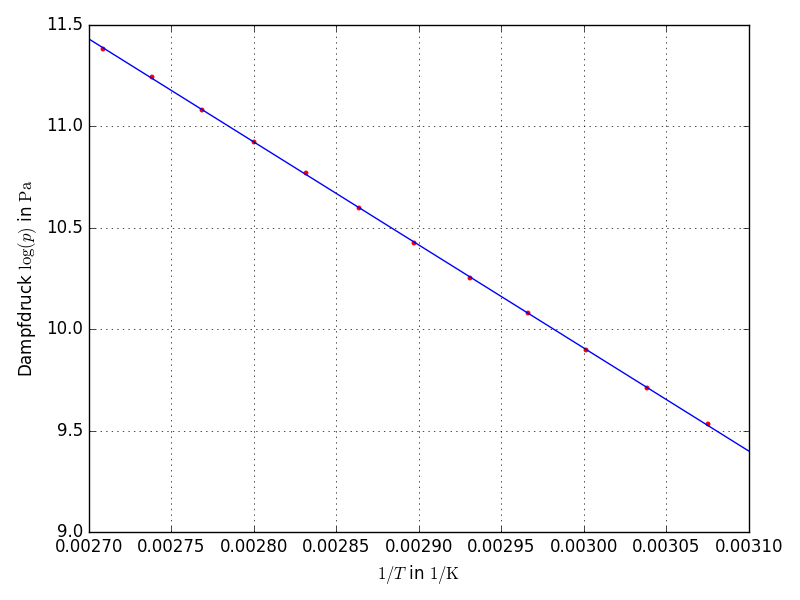
\includegraphics[width=\textwidth]{gerade.png}
  \caption{$p$ logarithmisch aufgetragen gegen die reziproke Temperatur $T$.}
  \label{fig:1}
\end{figure}

Mit dem idealen Gasgesetzt wird, unter der Annahme $T = \num{373}\si{\kelvin}$ , $L_a$ berechnet die äußere Verdampfungswärme
\begin{align*}
  L_a &= \frac{W}{n} = T\cdot R = \SI{373}{\kelvin}\cdot R = \SI{3,101e3}{\joule\per\mole}\\
  \intertext{und damit ergibt sich eine Abtrennarbeit zwischen den Atomen von}\\
  L_i &= L - L_a = \SI{4,223(12)e4}{\joule\per\mol} - \SI{3,101e3}{\joule\per\mole} =  \SI{3,912(12)e4}{\joule\per\mole}.\\
  \intertext{Damit ist dann die Abtrennarbeit pro Molekül }\\
  L_\text{i,molekular} &= L_i \cdot N_A = \SI{6,497(34)e-20}{\joule} = (\num{0,4055(21)})\mathrm{eV}.\\
\end{align*}

\subsection{Hochdruckmesung}
\label{sub:Hochdruckmesung}

Mit den Werten der zweiten Messung soll nun die Temperaturabhängigkeit der Verdampfungswärme bestimmt werden.

\begin{equation*}
  L = (V_D -V_F)\cdotT\cdot\frac{dp}{dT}
\end{equation*}
Wie zuvor ist $V_F$ zu vernachlässigen,
aber $V_D$ kann nicht mit dem idealen Gasgesetz genähert werden und muss jetzt berechnet werden durch
\begin{align*}
  (p(T)+\frac{a}{V_D^2})V_D &= RT \text{ mit } a = \SI{0,9}{\joule\meter\cubed\per\mole\squared}\\
  V_D &= \frac{RT}{2p(T)}+\sqrt{\frac{R^2T^2}{4p(T)^2}-\frac{a}{p(T)}}.
\end{align*}
Die Wurzel wird hierbei als positiv angenommen, da sich ansonsten eine Nullstelle ergeben könnte,
was dann negative Druckverläufe impliziert.
Für $p(T)$ und $\frac{dp}{dT}$ wird aus den Werten der Hochdruckmessung ein Ausgleichspolynom dritten Grades erstellt.

\begin{table}
\centering
\caption{Druck im Inneren des Gerätes (ca. 2,5 bar versetzt)}
\label{tab:Dicke}
\begin{tabular}{ S[table-format=3.0] S[table-format=2.1] }
\toprule
$ T/\si{\celsius}$ & $p/\si{\bar}$ \\
\midrule
100 &  -1,51 \\
102 &  -1,13 \\
104 &  -0,60 \\
106 &  -0,14 \\
108 &  0,33 \\
110 &  0,77 \\
112 &  1,24 \\
114 &  1,87 \\
116 &  2,47 \\
118 &  3,01 \\
120 &  3,65 \\
122 &  4,36 \\
124 &  5,17 \\
126 &  5,93 \\
128 &  6,81 \\
\bottomrule
\end{tabular}
\end{table}

Daraus ergibt sich dann das Näherungspolynom als 
\begin{align*}
  p(T) &= a_3\cdot T^3 + a_2\cdot T^2 + a_1\cdot T^1 + a_0\\
  \text{ mit }
  a_0 &= \SI{-5,6(12)e8}{\pascal}\\
  a_1 &= \SI{4,5(9)e6}{\pascal\per\kelvin}\\
  a_2 &= \SI{-1,19(23)e4}{\pascal\per\kelvin\squared}\\
  a_3 &= \SI{10,6(20)}{\pascal\per\kelvin\cubed}\\
\end{align*}


\begin{figure}
  \centering
  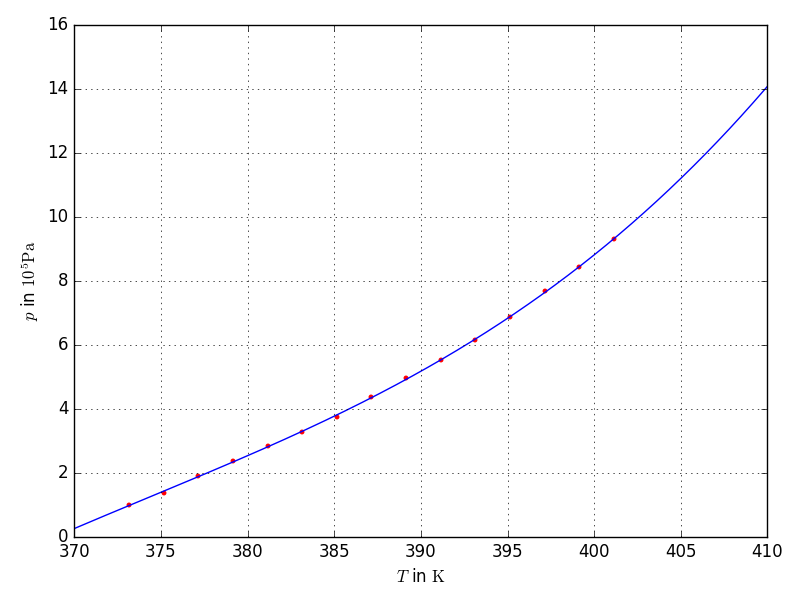
\includegraphics[width=\textwidth]{poly.png}
  \caption{Kubisches Ausgleichspolynom für die Werte der Hochdruckmessung.}
  \label{fig:pol}
\end{figure}

\begin{figure}
  \centering
  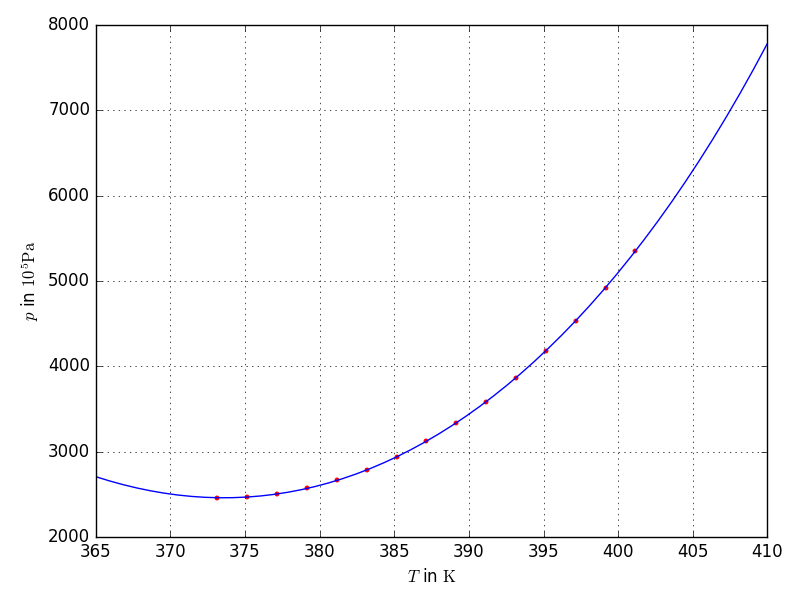
\includegraphics[width=\textwidth]{L(T).png}
  \caption{Verlauf der Verdampfungswärme $L(T)$ mit Ausgleichspolynom für p(T).}
  \label{fig:pol}
\end{figure}